\documentclass[a4paper,12pt]{article}
\usepackage{ucs}
\usepackage[utf8x]{inputenc}
\usepackage{amsfonts}
\usepackage[english,russian]{babel}
\usepackage[T1,T2A]{fontenc}
\frenchspacing
\usepackage{amsmath,amssymb,amsthm}
\usepackage[a4paper, margin=1in]{geometry}
\usepackage[table]{xcolor}
\usepackage{multirow}
\usepackage{diagbox}
\usepackage{graphicx}
\graphicspath{ {./} }

\newtheorem{name}{Printed output}
\newtheorem{problem}{Задача}
\newenvironment{solution}{\renewcommand{\proofname}{\unskip\indent\nopunct}\begin{proof}}{\end{proof}}

\begin{document}

\title{ДЗ 3}
\author{Витя\,Ефремов}
\maketitle

\begin{problem}
Монета подбрасывается 10 раз.
Найти вероятность p(k) выпадения орла k раз, где k = 0, 1, 2 \dots 10.
Проверьте, получается ли сумма вероятностей равной единице.
Постройте график функции p(k), соблюдая масштаб.
Соедините полученные точки плавной кривой.
\end{problem}
\begin{solution}
Это просто схема Бернулли.
Вероятности в таблице ниже.
Их сумма в точности равна 1.

\begin{tabular}{|c|c|}
\hline
k & p(k) \\
\hline
0 & 0.00098 \\
1 & 0.00977 \\
2 & 0.04395 \\
3 & 0.11719 \\
4 & 0.20508 \\
5 & 0.24609 \\
6 & 0.20508 \\
7 & 0.11719 \\
8 & 0.04395 \\
9 & 0.00977 \\
10 & 0.00098 \\
\hline
\end{tabular}
\\
\\
График вероятностей:

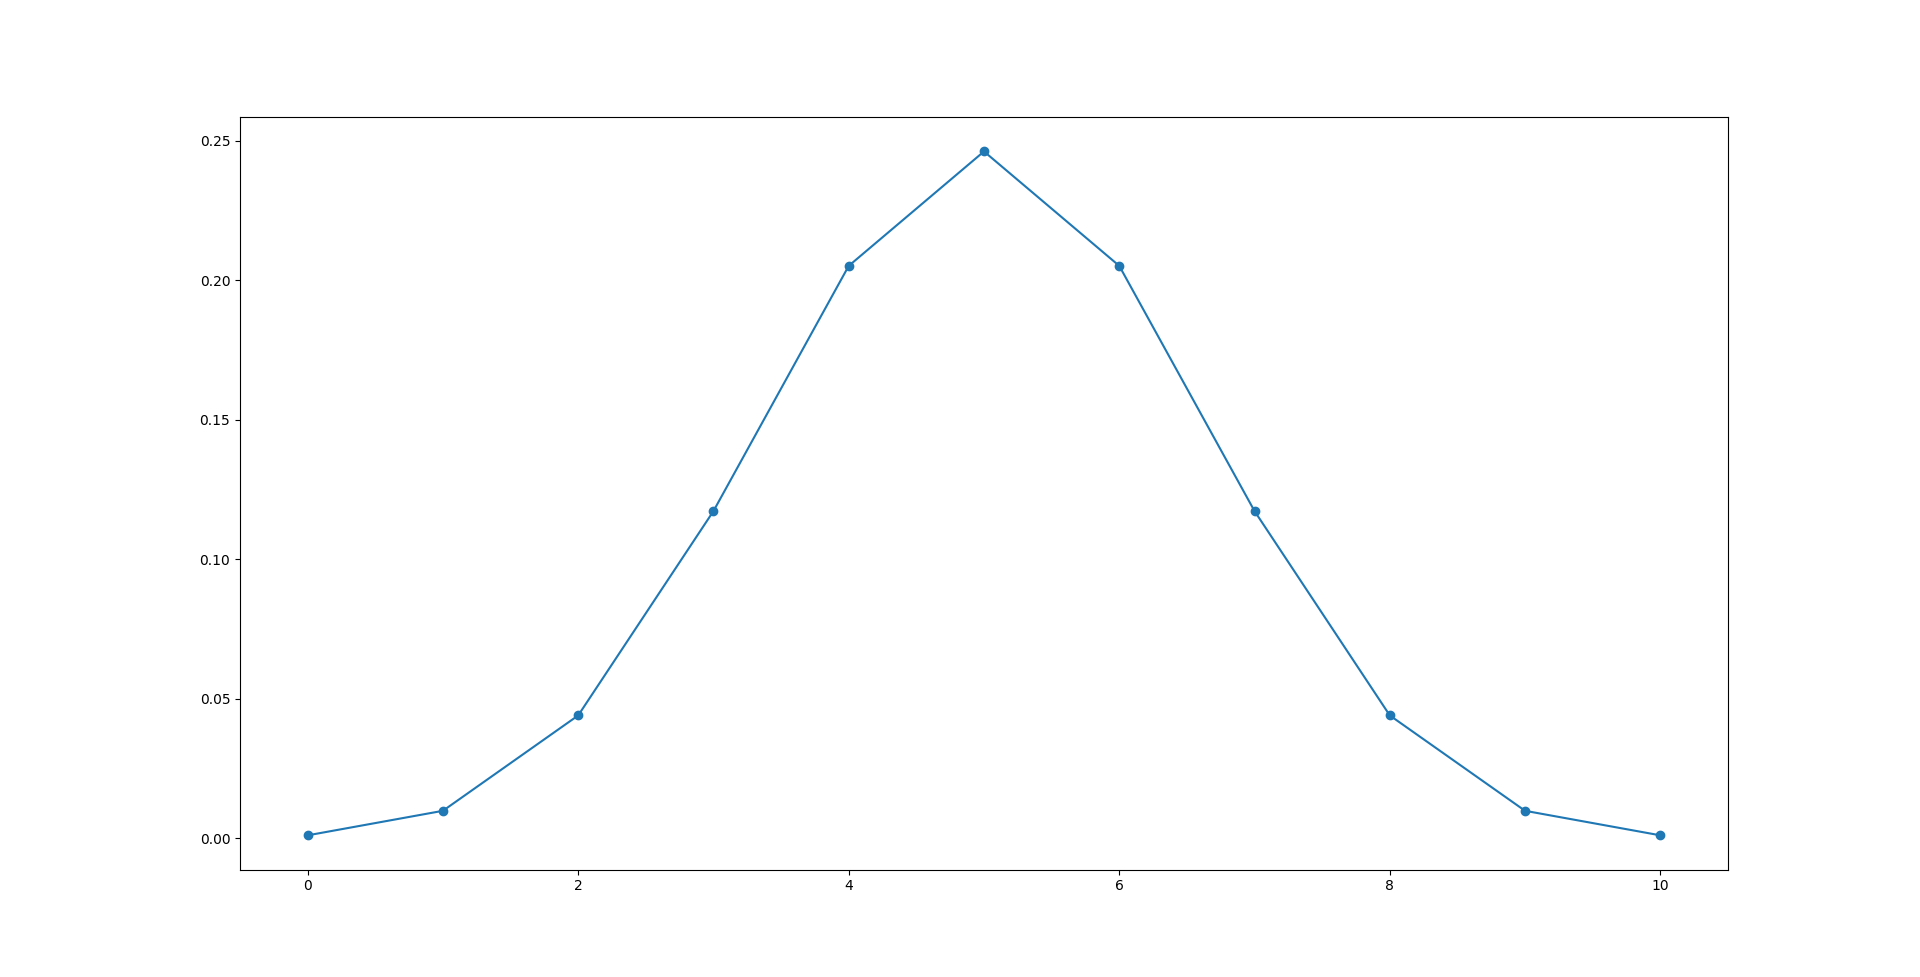
\includegraphics[width=\textwidth]{hw_3.1}

\end{solution}

\begin{problem}
В урне находятся 4 белых, 4 черных и 2 красных шара.
Из урны повторным способом выбирают семь шаров.
Какова вероятность того, что 3 раза будет выбран белый шар, 3 раза -- черный, и 1 раз -- красный?
\end{problem}
\begin{solution}
Воспользуемся обобщенной формулой Бернулли.
Пусть $A_1$ -- событие ``вытащили белый шар``, $A_2$ -- ``вытащили черный шар``, $A_3$ -- ``вытащили красный шар``.
Их вероятности -- $p_1 = 0.4, p_2 = 0.4, p_3 = 0.2$
Событие $A_1$ наступает $k_1 = 3$ раза, $k_2 = 3$, $k_3 = 1$ соответственно.
Итоговая вероятность $$P = \frac{(k_1+k_2+k_3)!}{k_1!\, k_2!\, k_3!} \cdot p_1^{k_1} p_2^{k_2} p_3^{k_3} = \frac{7!}{3!\,3!\,1!} \cdot 0.4^3\cdot0.4^3\cdot0.2^1 \approx 0.115$$
\end{solution}

\begin{problem}
На многоканальный телефон фирмы за 5 минут поступает в среднем один вызов.
Какова вероятность того, что 10 минут подряд вызовов не будет, а в следующие 5 минут поступят ровно два вызова?
\end{problem}
\begin{solution}
В среднем, частота звонков -- 1 в 5 минут.
Рассмотрим первые 10 минут без звонков и оставшиеся 5 минут с двумя звонками как отдельные, независимые события.
Вероятность, что за 10 минут не будет ни одного звонка $$p_1 = \frac{2^0}{0!} \cdot e^{-2}$$
А вероятность, что за 5 минут произойдет два звонка $$p_2 = \frac{1^2}{2!} \cdot e^{-1}$$
Итоговая вероятность -- просто произведение $$p = p_1\,p_2 \approx 0.0249$$
\end{solution}

\end{document}
